\chapter{Method}

\Large We have used Unity Engine to generate the buildings, roads, and trees which is capable of handling the 3D procedural model with help of L System model. The basic models likes cities, roads and tress models are in their default orientation, whenever any object is instantiated in the scene, checks with the neighbour objects and sync to them. For instance: roads are different because there are intersections, dead ends and 3 way roads. Everything is calculated and verified with their neighbours models which generated through L System model\cite{abrahamcity}.

\vspace{0.5cm}


\begin{wrapfigure}{l}{0.6\textwidth} %this figure will be at the right
    \caption{Flow chart of a L System model}
    \label{fig:flowchart}
    \centering
    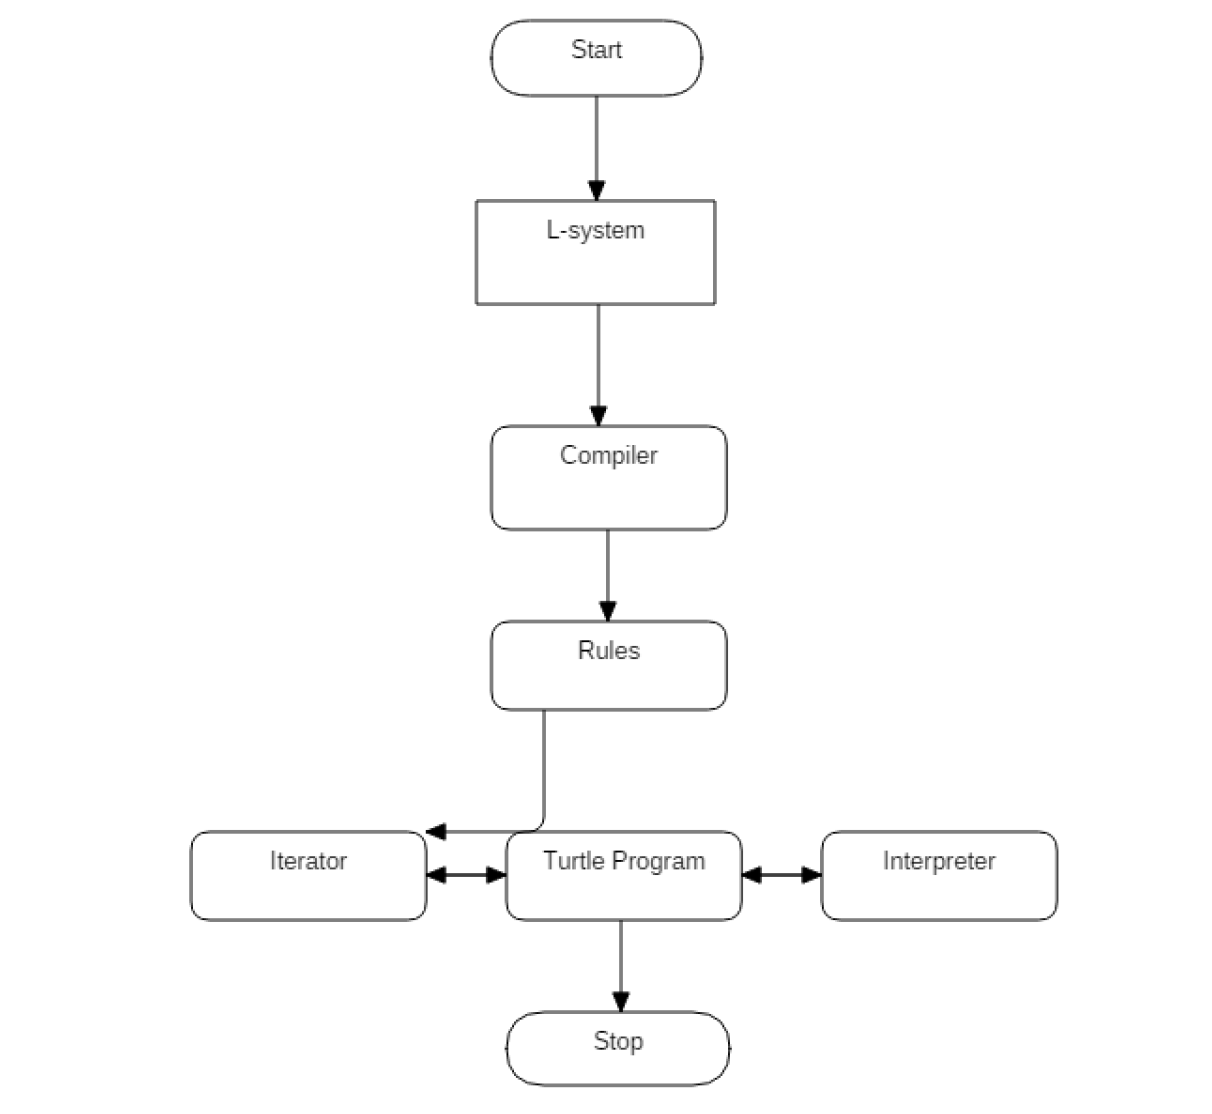
\includegraphics[width=0.6\textwidth]{3. method/Lsystem Flow Chart.png}
\end{wrapfigure}

\Large Buildings and trees are generated on bases of the road layout because they are needed to spawned beside the roads, similarly, trees are created with the equal subsequent distance among houses and also depends on the length of the street. The figure \ref{fig:flowchart} shows the flow of the model while generating it on run-time and described in the \cite{abrahamcity} an iterative process where graphics is interpreted with the strings. Some include of the stochastic rules a letter is replaced by the string with a probability of rules and angles.   



